\section{Costs and Other Details of Education} \label{appendix:education}

\noindent We account for short- and long-term components of education costs. The short-term components include savings due to reductions in special education and grade retention. The long-term components include the type and level of the highest educational attainment at age 30. We do not calculate costs of education beyond age 30 because we do not have data on it. Instead of forming a projection, we decide not to add further modeling uncertainty through this component and document that, at the national level, education beyond age 30 increases marginally---this holds true for a sample comparable to the ABC sample. To document this, we use the  Panel Study of Income Dynamics (PSID) for a representative sample of individuals born between 1972 and 1982. \\

\begin{figure}[H]
\begin{center}
\caption{High School and GED} \label{fig:hsorged}
\begin{subfigure}{.5\textwidth}
\subcaption{Female}\label{subfig:hs_stat_female}
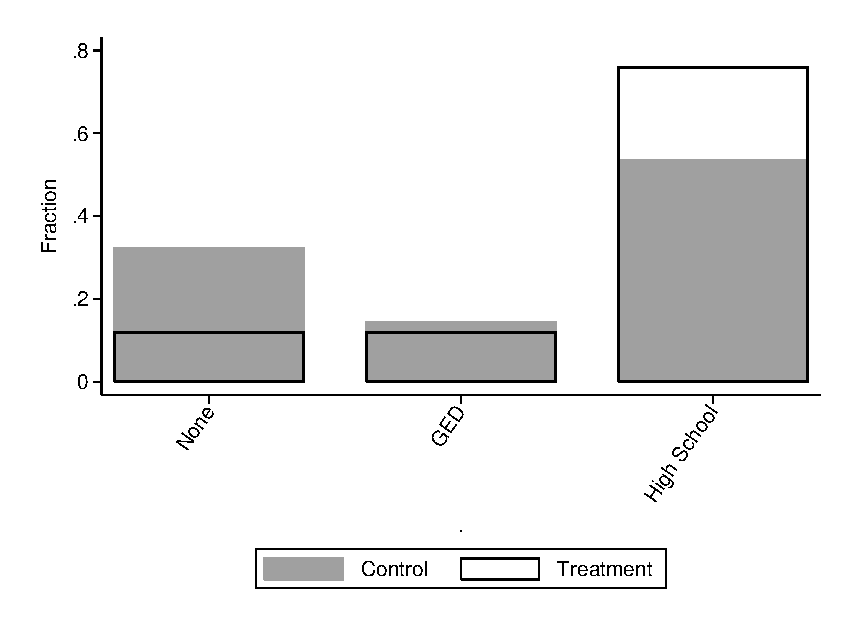
\includegraphics[height=2.5in]{AppOutput/Education/hsorged_female_age30.eps}
\end{subfigure}
\begin{subfigure}{.5\textwidth}
\subcaption{Male}\label{subfig:hs_stat_male}
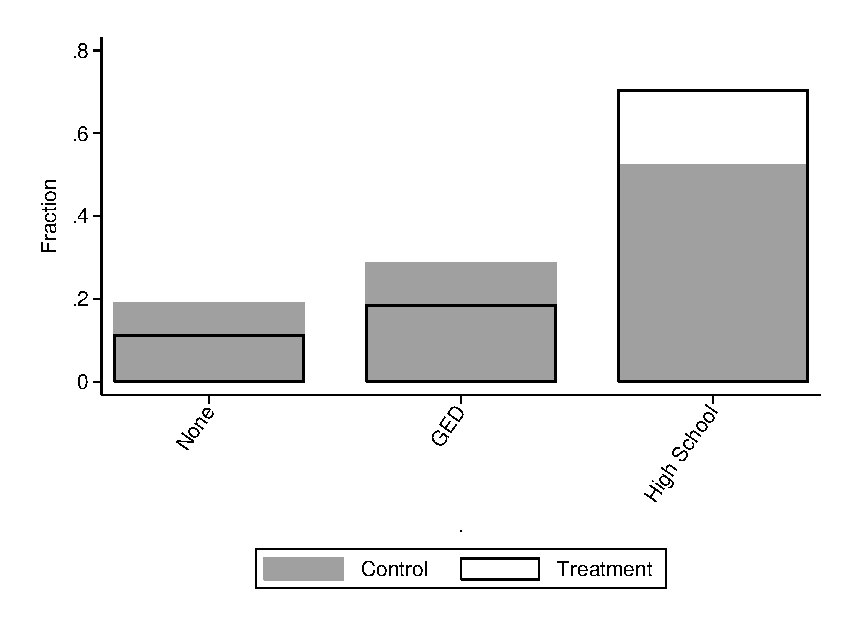
\includegraphics[height=2.5in]{AppOutput/Education/hsorged_male_age30.eps}
\end{subfigure}
{\footnotesize \flushleft Note: These plots display the fraction of individuals who finished high school, obtained a GED, or completed neither by treatment status. These categories are exclusive. Data are taken from self-reported measures at age 30. We have responses from 101 out of 111 individuals in the initial sample.\\}
\end{center}
\end{figure}

\noindent We document the benefits of additional schooling through increases in income or health in following sections. In this section we focus on the costs of additional schooling. The effects on total years of education and high school graduation are both statistically and economically significant. The effects on women are stronger. In Figure \ref{fig:hsorged} we note that treatment made a substantial difference between high-school- and GED-completion rates. This is a relevant component of the program's cost. \\

\noindent To estimate the costs of additional schooling, we combine various sources. Table \ref{tab:yearlyedu}   describes the yearly cost of education at every level and the age and duration for which these costs are incurred. We apply these costs additively up to the highest level of educational attainment by age 30. Pooling males and females, the treatment group had on average higher attainment and incurred a greater cost of education. To find the present value of the difference between the treatment and control groups, we first order educational attainment per Table \ref{tab:yearlyedu}. We find a difference between the average educational attainment of the treatment group (finish community college) and the average educational attainment of the control group (start community college). This can be represented as a cost that is \$12,586 higher for the treatment group than for the control group, as in Table \ref{tab:yearlyedu}. The effect of the program on females, however, is much greater than the effect on males.

\subsection{Measuring Lifetime Educational Attainment}

\noindent Follow-up data on educational attainment were collected for ABC subjects up to age 30, on average. This may not necessarily be an accurate measure of lifetime educational attainment. Thus, we perform an exercise using nationally representative data from the Panel Study of Income Dynamics (PSID) to assess educational attainment after age 30. Figure \ref{fig:psid-exercise} shows the results of our exercise. \\

\begin{figure}[H]
\caption{Additional Education After Age 30} \label{fig:psid-exercise}
    \centering
\begin{subfigure}{.5\textwidth}
  \centering
  \subcaption{PSID Yearly, All}\label{fig:psid-yearly-all}
  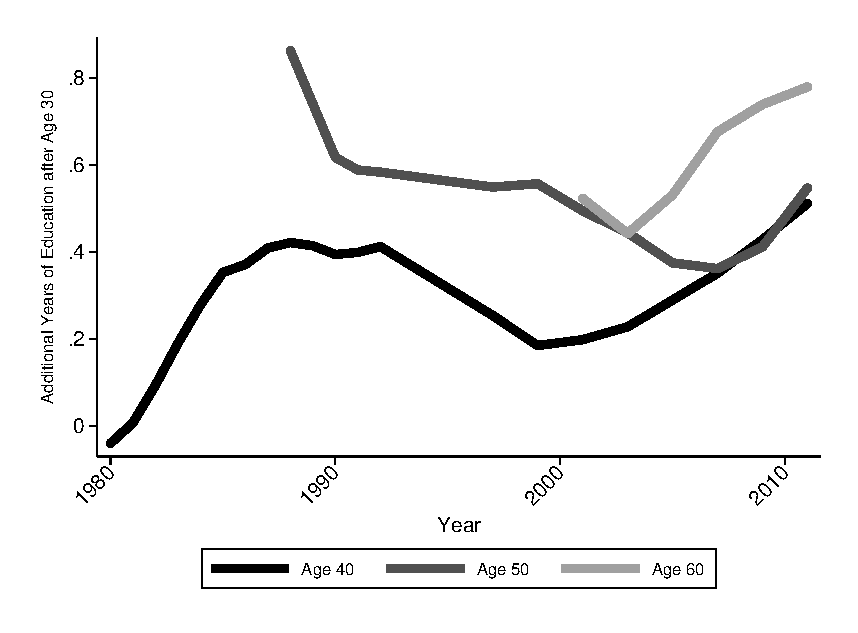
\includegraphics[height=2.5in]{AppOutput/Education/addeducfrom30.eps}
\end{subfigure}%
\begin{subfigure}{.50\textwidth}
  \centering
  \subcaption{ABC-Eligible PSID Educational Attainment by Age}\label{fig:abc-psid-sample}
  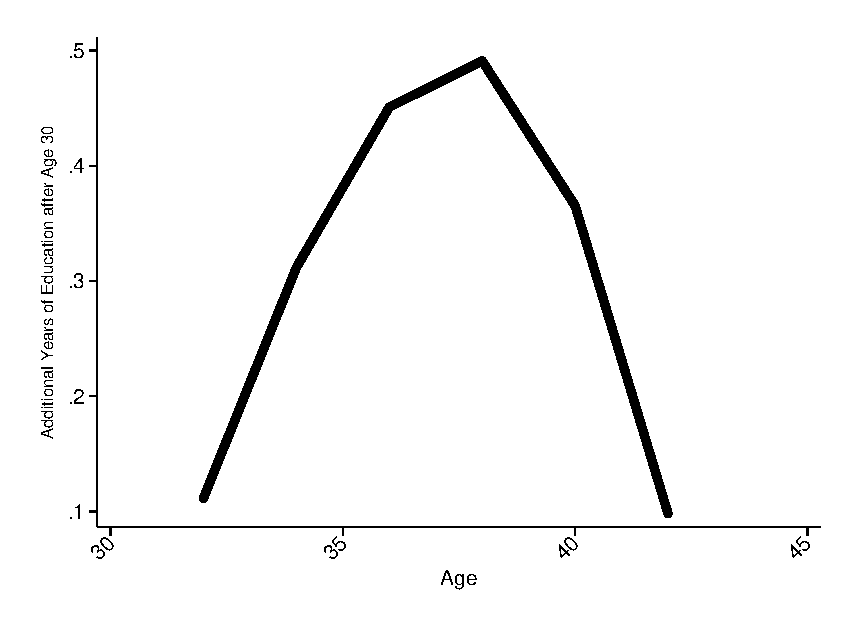
\includegraphics[height=2.5in]{AppOutput/Education/addeducfrom30matched.eps}
\end{subfigure}
\floatfoot{
\scriptsize
Note 1 (left panel): this plot uses data from the Panel Study of Income Dynamics (PSID) to display the mean years of education beyond the education level at age 30, by years. We report this value for ages 40, 50, and 60. The domain of the trends is a function of data availability, i.e. of longitudinal span in the data. Each yearly calculation uses cross-sectional weights to attain nationally representative statistics. \\
Note 2 (right panel): this plot uses a restricted sample of the PSID. We only consider individuals who would have been eligible to ABC following the procedure in \citet{Garcia_Heckman_2014_AbilityCharacter}. We pool all the years and plot the mean years of education beyond the education level at age 30, by age.
}
\end{figure}

\noindent Figure~\ref{fig:psid-yearly-all} displays the average additional years of education at ages 40, 50, and 60. The series have different spans due to restrictions in data availability. Figure~\ref{fig:abc-psid-sample} uses a sample of individuals that would have been eligible to be part of ABC. Furthermore, we restrict the sample to the 1972--1982 cohort of PSID, to mimic the ABC sample. To find the eligible sample we follow the same procedure as \citet{Garcia_Heckman_2014_AbilityCharacter}. Broadly, we reconstruct the ABC eligibility index in the PSID and construct a sample of ``ABC-eligible individuals.'' The data availability is not enough to perform a yearly analysis. We pool all the available years to construct this plot---roughly, 1990 to 2010. Both plots show that individuals, on average, never go a year beyond their education at age 30. We assume that imprecision generated by not observing educational levels beyond age 30 is of second order. \\


\subsection{Treatment Effects on Education}
\noindent To analyze the long-term impact of ABC on educational attainment,
we examine data on grade retention, special education, and
years/type of schooling through 30 years of age. After 30,
educational attainment remains essentially
unchanged.%
	\footnote{Our calculation is based on
	the data from the Panel of Study of Income Dynamics (PSID) for a
	population born between 1972 and 1982 (the same age group as that of
	ABC participants). The data show that on average, the mean years spent
	on  education beyond age 30 was less than one year.
	Therefore, any potential concerns regarding uncertainties of our analysis
	by not observing educational levels beyond age 30 is second
	order.}
The benefits of additional schooling, e.g. through
increased income and improved health, is assessed in
subsequent sections. Here we focus on estimating the
differences in schooling costs between the treatment and
control groups. \\

\subsection{Cost of Education}
\noindent We apply the costs described in Table \ref{tab:yearlyedu} to subjects' educational attainment at age 30 to calculate the public and private costs of lifetime educational attainment. Costs up to high school are assumed to be public costs. \\

\begin{table}[H]
\caption{Yearly Individual Education Costs} \label{tab:yearlyedu}
\centering
\begin{adjustbox}{max width=\textwidth}
\begin{threeparttable}
\footnotesize
\begin{tabular}{C{3.5cm} C{1.5cm} C{1.5cm} C{2cm} C{6.5cm}}
\toprule
Schooling level & Ages & Duration (Years) & Yearly Cost &Attainment \& Notes\\ \midrule
K-11 & 6-16 & 10 &   \$9,113  & All subjects. Only 1 control individual dropped out before completing 9th grade; we assume completion up to 8th grade. \\
Grade 12 & 17-18 & 2 &  \$9,113  & Counted only for subjects who completed high school, 29:38 (control:treatment).\\ \\
GED (Started) & 19 & .5 &  \$155& GED is considered a one year program. No subjects identified as having starting a GED program without finishing.\\ \\
GED (Completed) & 19 & 1 & \$155 & 8:6 (control:treatment).\\ \\
Vocational or Technical Training (Started)& 19 & 1 & \$7,245 & 8:3  (control:treatment).\\ \\
Vocational or Technical Training (Completed)& 19-20 & 2 &  \$7,245 &  4:9 (control:treatment)\\ \\
Community College (Started) &   19 & 1 &  \$7,001 & 11:6 (control:treatment) \\ \\
Community College (Completed) & 19-20 & 2 &  \$7,001 & 9:8 (control:treatment)\\ \\
 College (Started)   &  19 & 1 &  \$7,685& Assume dropouts drop out at the end of the first year. 5:8 (control:treatment).\\ \\
 College (Completed) &  19-22 & 4 & \$11,886 & 3:8 (control:treatment)\\ \\
Graduate School (Started) & 23 & 1 &  \$9,704& Assume dropouts drop out at the end of the first year. 2 treated individuals.\\ \\
 Finished Masters &  23-25 & 2 &  \$9,704& 1 treated individual\\ \\
 Finished PhD & 23-26 & 4 & \$9,704 & 1 treated individual\\ \\
 \midrule
 Grade Retention& NA & 1 &\$9,113 & \\ \\
 Special Ed.& NA & 1 &  \$11,705  & \\ 
 \bottomrule
 \end{tabular}

\centering
\begin{tablenotes}%[para,flushleft]
\scriptsize
\item Sources: \citet{Snyder_Willow_2012_BOOK_NCES}; \citet{Hoenack_Weiler_1975_JHR}; \cite{Dhanidina_Griffith_1975_AEQ}; \cite{Freeman_1974_Occupational-Training_RES}. \\
 Note: this table reports the yearly cost and duration of each type of education, as well as the ages for which we evaluate them.  All amounts are inflated to 2014 USD.
We show the number of respondents who identified themselves as being in each education category (total number of respondents: 101/114). To compute the total cost of education for an individual, we applied these costs additively up to the highest level of educational attainment. Only K-12 education, special  education, and grade retention costs account for deadweight loss. Because it gives costs that are applied across many years, this table does not show their present discounted value.
\end{tablenotes}
\end{threeparttable}
\end{adjustbox}
\end{table}


\subsection{Non-monetary Benefits of Education}

\noindent There are many social and non-monetary benefits of education that our analysis cannot capture. These benefits impact the individual's quality of life, the general well-being of society through positive peer effects as well as fewer costs and negative externalities, and even the well-being of future generations. Documenting them all may be impossible, but we briefly review some major benefits in this section. \cite{Vila_2000_Non-Monetary-Benefits-Education} documents private benefits with external effects, such as health (increases in longevity and better nutrition and preventative care choices). Higher education is also associated with decreased fertility rates linked with improved infant health and mortality rates. Moreover, higher education not only improves labor outcomes with respect to employment prospects and salary, but also with regard to how individuals perceive work and leisure, with more education leading to increased satisfaction from leisure. Furthermore, higher education is linked with better savings behavior and higher rates of return on savings. Higher education is also connected with social stability---better education promotes good citizenship and creates communities that are less likely to experience violent social conflict.\footnote{\citet{Lochner_2011_Handbook} or \citet{Lochner_2011_NBER}.} \\